\documentclass[11pt]{article}

\usepackage{amsmath}
\usepackage{amssymb}
\usepackage{enumitem}
\usepackage[final]{graphicx}
\graphicspath{{./project_structure.pdf}}
\usepackage{xurl}
\usepackage{float}

\usepackage{fontspec}
\newfontfamily{\lean}[Scale=MatchLowercase]{Consolas}
\newfontfamily{\ftl}[Scale=MatchLowercase]{DejaVuSansMono}

\usepackage{color}
\definecolor{leanBlue}{RGB}{86,156,214}
\definecolor{leanYellow}{RGB}{179,160,0}
\definecolor{ftlComment}{RGB}{204,0,0}
\definecolor{ftlRead}{RGB}{255,132,0}
\definecolor{ftlSignature}{RGB}{0,102,153}
\definecolor{ftlProof}{RGB}{0,153,255}
\definecolor{ftlAssume}{RGB}{0,153,102}

\usepackage{textgreek}
\usepackage{listings}

\lstdefinelanguage{Lean}{
  keywords=[1]{class, lemma, theorem, lemma, def, by, at, include, @[simp], end, Type, Prop, extends, universe, universes, variable, variables, namespace, import},
  keywordstyle=[1]{\color{leanBlue}},
  morestring=[s][\color{leanBlue}]{@[}{]},
}
\lstdefinestyle{lean}{
	language={Lean},
    basicstyle=\lean\footnotesize,
    breakatwhitespace=false,
    breaklines=true,
    captionpos=b,
    keepspaces=true,
    numbers=none,
    showspaces=false,
    showstringspaces=false,
    showtabs=false,
    tabsize=2,
    breakindent=10pt,
    frame=trbl,
    frameround=tttt,
    framesep=3pt,
    mathescape=true,
    escapeinside={§}{§},
}

\lstdefinelanguage{ForTheL}{
  keywords=[1]{Signature, Axiom, Theorem, Definition},
  keywords=[2]{Proof, End, qed, by},
  keywords=[3]{and, Assume, Let, Since, we, have},
  sensitive=false,
  keywordstyle=[1]{\color{ftlSignature}},
  keywordstyle=[2]{\color{ftlProof}},
  keywordstyle=[3]{\color{ftlAssume}},
  morestring=[s][\color{ftlRead}]{[read}{]},
  morestring=[s][\color{ftlRead}]{[synonym}{]},
  morestring=[s][\color{ftlAssume}]{Let\ us\ show}{that},
  morecomment=[l]{\#},
  commentstyle={\color{ftlComment}},
}
\lstdefinestyle{ftl}{
    language={ForTheL},
    basicstyle=\ftl\footnotesize,
    breakatwhitespace=false,
    breaklines=true,
    captionpos=b,
    keepspaces=true,
    numbers=none,
    showspaces=false,
    showstringspaces=false,
    showtabs=false,
    tabsize=2,
    breakindent=0pt,
    frame=trbl,
    frameround=tttt,
    framesep=3pt,
    escapeinside={§}{§},
}


\author{Erik Sturzenhecker, Felix Thiele}
\title{A Start to the formalization of Linear Algebra in ForTheL}
\date{\today}


\begin{document}
\maketitle
\newpage 
\setcounter{tocdepth}{10}
\tableofcontents

\newpage 
\section{Introduction}
\subsection{Naproche}
In this project we build a linear algebra library in ForTheL with Naproche-SAD. ForTheL, which stands for Formal Theory Language, is a language that comes close to human language. This reduces many of the initial hurdles people encounter in the formalization of mathematics. Naproche can not only interpret ForTheL code, but is also backed with a strong automated theorem prover, to which we shall refer to as e-prover. This makes many proofs in our library easier, since some trivial steps can be skipped. At the same time this comes with massive performance issues, since checking this small library is a comparably very time intensive task.

\subsection{Results}
The complete project can be found under \url{https://github.com/Felix-Thiele/linear_algebra_ftl}.
Some of the results given in this library are:
\newline
The \textbf{definitions} of:
\begin{itemize}[nolistsep, noitemsep]
\item groups, rings, fields
\item vector spaces, subspaces, dual spaces
\item homomorphisms, endomorphisms, automorphisms of vector spaces
\item lists, linear independence
\end{itemize}
And the \textbf{proofs} of:
\begin{itemize}[nolistsep, noitemsep]
\item A field is a vector space over itself.
\item The linear maps between $K$-vector spaces $V$ and $W$ form a vector space Hom($K$,$V$,$W$).
\item If $f$ is linear, Ker($f$) is a subspace.
\item If $f$ is linear and Ker($f$) $=$ \{0\}, then $f$ is injective.
\item Any $K$-vector space $V$ can be embedded into the double dual space $(V^{*})^{*}$
\item The endomorphisms of a $K$-vector space $V$ form a ring End($K$,$V$).
\item The invertible elements of a ring form a multiplicative group.
\end{itemize}


\newpage
\lstset{style=lean}
\section{The Lean File}
For inspiration on how to formalize linear algebra for a proof checker, we looked into the file "vector\_space.lean" found under \url{https://github.com/kckennylau/Lean/blob/master/linear_algebra/vector_space.lean}. It is part of a small Lean library by Kenny Lau containing formalizations of various mathematical topics. Lean is a theorem prover and a programming language based on dependent type theory. There is an extensive library of mathematical Lean texts, the mathlib (\url{https://github.com/leanprover-community/mathlib}), maintained by Lean users, which is used and build upon in vector\_space.lean.



\subsection{Mathematical Content} \label{mathematicalContent}
The file vector\_space.lean covers the following definitions and statements of linear algebra:
\begin{itemize}
\item {\lean field.to\_vector\_space}: Any field is a vector space over itself.
\item {\lean sub\_vector\_space}: Definition of a vector subsace. Definition and proof of the vector space structure on it.
\item {\lean linear\_space K V W}: Definition of the set of linear maps between two $K$-vector spaces $V$ and $W$. Easy proofs about linear maps.
\item {\lean ker}: Definition of the kernel of a linear map. Some small proofs.
\item Definition and proof of the vector space structure on {\lean linear\_space K V W}.
\item Definition of the dual vector space.
\item Definition and proof of the ring structure on {\lean linear\_space K V V} by taking the function composition as multiplication.
\item {\lean invertible K V}: Definition and proof of the (general linear) group structure on the invertible elements of {\lean linear\_space K V V}
\end{itemize}


%
\subsection{Characteristic Features} \label{characteristics}
The notions above are defined in the canonical way and the proofs are of course trivial from an algebraic standpoint. Thus, there is no need for huge lambda terms (which are otherwise not uncommon in Lean texts) and the code is fairly easy to understand.

The Lean file uses the following notions (type classes) from the mathlib: {\lean field}, {\lean discrete\_field} (a field where equality of elements is decidable), {\lean add\_comm\_group}, {\lean vector\_space}, {\lean ring}, {\lean group}.
The classes {\lean has\_zero}, {\lean has\_one}, {\lean has\_add}, {\lean has\_mul}, {\lean has\_neg}, {\lean has\_inv}, {\lean has\_scalar} from the built-in lean library are crucial for the description and handling of algebraic structures in Lean.
The following is an example of how algebraic structures are successively defined as type classes in the mathlib, by extending existing type classes:
\begin{lstlisting}
universe u

class §\textcolor{leanYellow}{has\_zero}§ (§\textalpha§ : Type u) := (zero : §\textalpha§)
class §\textcolor{leanYellow}{has\_add}§  (§\textalpha§ : Type u) := (add : §\textalpha§ → §\textalpha§ → §\textalpha§)
class §\textcolor{leanYellow}{has\_neg}§  (§\textalpha§ : Type u) := (neg : §\textalpha§ → §\textalpha§)

class §\textcolor{leanYellow}{add\_semigroup}§ (§\textalpha§ : Type u) extends has_add §\textalpha§ :=
(add_assoc : $\forall$ a b c : §\textalpha§, a + b + c = a + (b + c))

class §\textcolor{leanYellow}{add\_comm\_semigroup}§ (§\textalpha§ : Type u) extends add_semigroup §\textalpha§ :=
(add_comm : $\forall$ a b : §\textalpha§, a + b = b + a)

class §\textcolor{leanYellow}{add\_monoid}§ (§\textalpha§ : Type u) extends add_semigroup §\textalpha§, has_zero §\textalpha§ :=
(zero_add : $\forall$ a : §\textalpha§, 0 + a = a) (add_zero : $\forall$ a : §\textalpha§, a + 0 = a)

class §\textcolor{leanYellow}{add\_comm\_monoid}§ (§\textalpha§ : Type u) extends add_monoid §\textalpha§, add_comm_semigroup §\textalpha§

class §\textcolor{leanYellow}{add\_group}§ (§\textalpha§ : Type u) extends add_monoid §\textalpha§, has_neg §\textalpha§ :=
(add_left_neg : $\forall$ a : §\textalpha§, -a + a = 0)

class §\textcolor{leanYellow}{add\_comm\_group}§ (§\textalpha§ : Type u) extends add_group §\textalpha§, add_comm_monoid §\textalpha§
\end{lstlisting}


Especially useful for algebraic proofs is the Lean tactic {\lean simp} (simplify). Easy statements like the ones mentioned in \ref{mathematicalContent}, which help with term rewriting, can be added to this tactic via {\lean @[simp]}:
\begin{lstlisting}
variables {K V W : Type} [discrete_field K] [add_comm_group V]
	[vector_space K V]

@[simp] def §\textcolor{leanYellow}{ker}§ (A : linear_space K V W) : V → Prop := (§\textcolor{leanBlue}{\textlambda}§ v, A.T v = 0)

@[simp] lemma §\textcolor{leanYellow}{map\_neg}§ : A.T (-v) = -(A.T v) :=
eq_neg_of_add_eq_zero (by {rw [←map_add], simp})

@[simp] lemma §\textcolor{leanYellow}{map\_sub}§ : A.T (u-v) = A.T u - A.T v := by simp
\end{lstlisting}
This allows for omitting detailed chains of equations and instead let {\lean simp} find the proof details automatically:
\begin{lstlisting}
theorem §\textcolor{leanYellow}{ker\_neg}§ (HV : A.ker v) : A.ker (-v) :=
by {unfold ker at *, simp [HV]}

theorem §\textcolor{leanYellow}{ker\_sub}§ (HU : A.ker u) (HV : A.ker v) : A.ker (u - v) :=
by {unfold ker at *, simp [HU,HV]}
\end{lstlisting}
Being able to tell lean which statements to use in the {\lean simp} tactic, while everything else has to be directly referenced, gives a performance advantage.

\subsection{Adjusting the Code}
The latest version of vector\_space.lean was from November 2017. Since then, it seems that the mathlib has developed to a point where it became incompatible with vector\_space.lean.
However, slight adjustments in the file made it work with the current version of the mathlib. This comprises the following changes:
\begin{itemize}
\item While the original file used {\ftl [field K]} as the only assumption for working with a {\ftl vector space K V}, we had to change this to {\lean [discrete\_field K]}. Also, the mathlib definition of a vector space now requires that V is already an abelian group, so we added {\lean [add\_comm\_group V]} as a second assumption at the same places.
\item We renamed {\lean subspace} to {\lean sub\_vector\_space}, since the name conflicted with the (apparently new) mathlib definition of a vector subspace.
\item The mathlib change described in the first point also demanded changes in places where objects like the {\lean linear\_space K V W} are proven to be a vector space over K: We had to cut parts from the old proof of the object being a vector space and pasting them into a new preceding proof of it being an abelian group. 
\item We adopted the mathlib renamings of {\lean smul\_left\_distrib} and {\lean smul\_ right\_distrib} to {\lean smul\_add} and {\lean add\_smul}, respectively. These are fields of the structure {\lean module.core}.
\item Some minor syntactical changes.
\end{itemize}
We could determine these necessary changes by looking at the underlying parts of the mathlib as well as the errors and proof states displayed in the "Lean Goal" window. Our final version of the file can be found under \url{https://github.com/Felix-Thiele/linear_algebra_ftl/blob/master/vector_space.lean}.



\newpage
\lstset{style=ftl}
\section{Formalization in ForTheL}
\subsection{Project Structure}
Giving the project a treelike structure with a file to each topic ensures increased readability and scalability. 
In contrast to having one large file building up mathematics, this enables us to pick what files need to be imported to each file. 
Our structure is depicted in the graph below.

\begin{figure}[h]
\begin{center}
\makebox[\linewidth][c]{
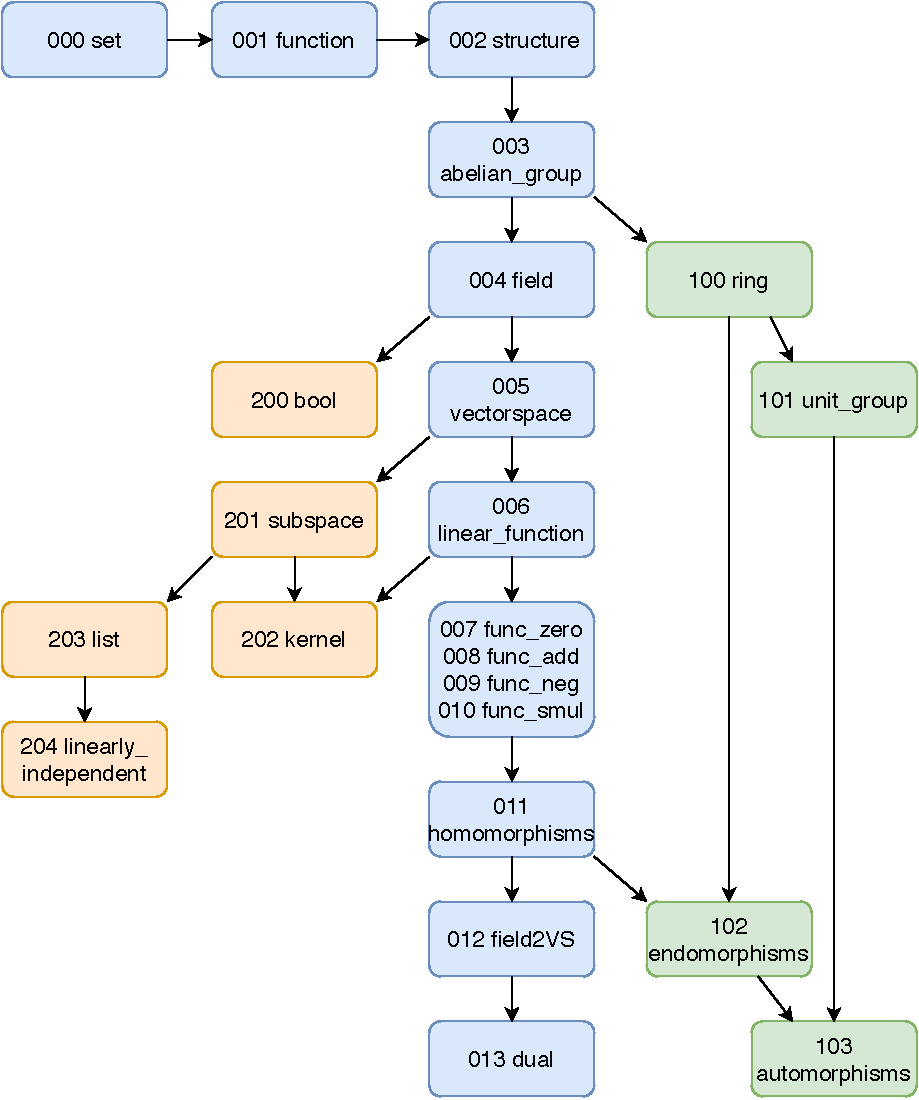
\includegraphics[scale=0.75]{./project_structure.pdf}
}
\end{center}
\end{figure}

\newpage

The e-prover is not fast enough to compile the entire library with all proofs in reasonable time. 
Instead, for every file we introduce two new files inserting "A\_" and "P\_" respectively in front of the file names. We insert "D\_" before our original file. This gives us an Axiom, Proof and Definition file. 
The Definition file holds all the definitions of the given topic. 
The Proof file holds the theorems and their proofs. The Axiom file holds all the statements of the Proof file in axiomatized form. 
The Proof and Axiom files only read their corresponding Definition file, while Definition files read the Axiom files of all the topics they are building upon. 
This ensures a fast compilation since we don't need to reprove proven statements. 
This file reading structure is depicted below.

\begin{figure}[h]
\begin{center}
\makebox[\linewidth][c]{
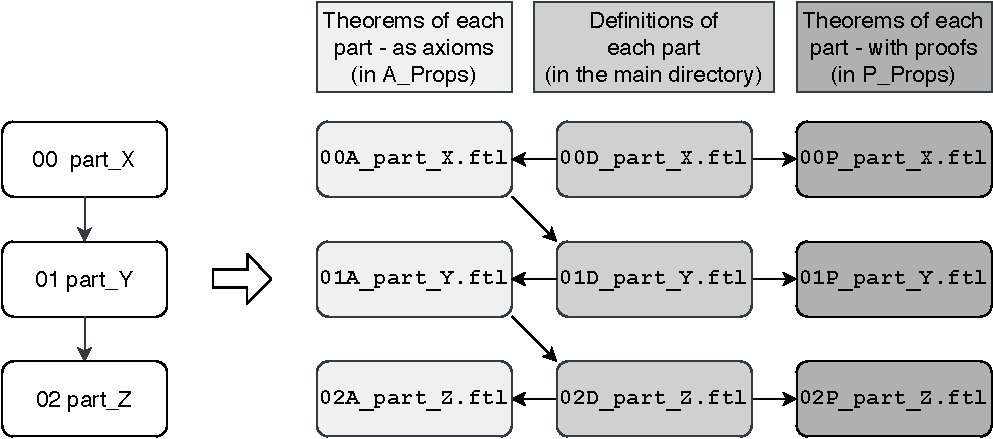
\includegraphics[scale=0.75]{./project_structure_explained.pdf}
}
\end{center}
\end{figure}

Additionally, it can sometimes be helpful to split the P\_ files even more, especially when more multiple theorems are supposed to follow on a single D\_ file. In our case, P\_vector\_space contained five (partly independent) theorems, each needing some lemmas. Reasoning and ontological checking of the proofs became considerably slower when the respective theorem was preceded by other lemmas and theorems. The solution was to write four different proof files (P\_vector\_space\_1, \_2, \_3 and \_4), each starting with only the required statements of the preceding proof files - in axiomatized form.


\subsection{The Implementation}

\subsubsection{Sets and Functions}

Our D\_ Set and D\_ Function files our kept very lightweight and only include key statements. This is due to both files being so close to the root node of the library graph. Adding more definitions will substantially slow down the e-prover in all following files.

\subsubsection{Algebraic Structures} \label{algebraicStructures}
Many of the objects we examine in this library have a similar structure. For example, abelian groups, fields, vector spaces and rings all have a carrier, a zero element, and an addition operation. We introduce an object called structure in 002D\_structure.ftl.
\begin{lstlisting}
Signature. lang is a set.
Axiom. lang = {carr,zero,one,add,mul,neg,inv,smul}.
Definition. A structure is a function S such that Dom(S) is subset of lang.
\end{lstlisting}


We can now define a each of the linear algebra structures above as a structure with the necessary components of {\ftl lang} in its domain. This allows for easy expansions of these structures one example of which we shall see in \ref{field2VS}. Now we define the following abbreviations:
\begin{lstlisting}
Let |S| stand for S[carr].
Let 0{S} stand for S[zero].
Let 1{S} stand for S[one].
Let add{S} stand for S[add].
Let mul{S} stand for S[mul].
Let neg{S} stand for S[neg].
Let inv{S} stand for S[inv].
Let smul{S} stand for S[smul].

Let a +{S} b stand for add{S}[(a,b)].
Let a *{S} b stand for mul{S}[(a,b)].
Let ~{S} a stand for neg{S}[a].
Let a -{S} b stand for add{S}[(a,neg{S}[b])].
Let a /{S} b stand for mul{S}[(a,inv{S}[b])].
Let a @{S} b stand for smul{S}[(a,b)].
Let a < S stand for a << |S|.
Let a < S* stand for a << |S|\{0{S}}.

Let (S has a) stand for (a << Dom(S)).
Let (S has a,b) stand for (a,b << Dom(S)).
...
Let (S has a,b,c,d,e,f,g,h) stand for (a,b,c,d,e,f,g,h << Dom(S)).
\end{lstlisting}

This approach resembles the notion of a structure in first-order logic: Our {\ftl structure} is the interpretation of (a subset of) the language {\ftl lang}, consisting of a set (if {\ftl |S|} is defined to be a set), constants and functions (if {\ftl zero}, {\ftl add}, etc. are defined to be suchlike).
This is done, for example, in the following definition of an abelian group, additionally postulating the corresponding (first-order) axioms:
\begin{lstlisting}
Definition. An abelian group is a structure G such that
     (G has carr,zero,add,neg)
 and (|G| is a set)
 and (0{G} < G)
 and (add{G} is a function from Prod(|G|,|G|) to |G|)
 and (neg{G} is a function from |G| to |G|)
 and (for all a < G     :       a +{G} 0{G} = a)
 and (for all a < G     :          a -{G} a = 0{G})
 and (for all a,b,c < G : a +{G} (b +{G} c) = (a +{G} b) +{G} c)
 and (for all a,b < G   :          a +{G} b = b +{G} a). 
\end{lstlisting}


\subsubsection{Homomorphisms}
After the definition of various algebraic structures, we define linear maps between vector spaces.
We introduce the set of homomorphisms as the carrier set of a new structure {\ftl Hom(K,V,W)}.
\begin{lstlisting}
Let K denote a Field.

Definition. Let V and W be vector spaces over K. Let f be a function.
 f is linear over K from V to W iff
     (f is from |V| to |W|)
 and (for all u,v < V             : f[u +{V} v] = f[u] +{W} f[v])
 and (for all a < K for all v < V : f[a @{V} v] = a @{W} f[v]).

Signature. Let V and W be vector spaces over K.
Hom(K,V,W) is a structure.

Axiom. Let V and W be vector spaces over K.
(Hom(K,V,W) has carr).

Axiom. Let V and W be vector spaces over K.
|Hom(K,V,W)| is the set of functions f such that f is linear over K from V to W.
\end{lstlisting}

Regarding this structure as a vector space requires quite an extensive preparation, which is done in the func\_ files, defining the zero, addition, negation, and scalar multiplication on {\ftl Hom(K,V,W)}. These are split from the D\_homomorphisms file because the corresponding P\_ files hold long proofs which become easier to check separately.
For brevity, in D\_func\_zero we introduce the following abbreviation:
\begin{lstlisting}
Let 2Vectorspace(K,V,W) stand for
(K is a field and (V is a vector space over K) and (W is a vector space over K)).
\end{lstlisting}

The {\ftl structure} approach allows us to also regard {\ftl Hom(K,V,W)} as a ring, which is done in the files about endomorphisms.

\subsubsection{Field2VS} \label{field2VS}
Proving that a field is a vector space over itself becomes again easy through the structure construction. We don't have to redefine the part of the structure that already exists but can instead just add scalar multiplication to the field. This is done in the following way:
\begin{lstlisting}
Let K denote a field.
Axiom. (K has smul).
Axiom. smul{K} = mul{K}.
\end{lstlisting}
We then prove in P\_field2VS that this really does create a vector space:
\begin{lstlisting}
Theorem. Let K be a field. Then K is a vector space over K.
proof.
 (K has carr,zero,add,neg,smul).
 K is an abelian group.
 smul{K} is a function from Prod(|K|,|K|) to |K|.
 For all u < K                 :       1{K} @{K} u = u.
 For all a,b < K for all v < K : (a *{K} b) @{K} v = a @{K} (b @{K} v).
 For all a,b < K for all v < K : (a +{K} b) @{K} v = (a @{K} v) +{K} (b @{K} v).
 For all a < K for all v,w < K : a @{K} (v +{K} w) = (a @{K} v) +{K} (a @{K} w).
qed.
\end{lstlisting}


\subsubsection{Automorphism Group}
While the Lean file introduces the general linear group by proving statements about invertible linear maps, we took a step back and defined the multiplicative group of an arbitrary ring in D\_unit\_group. This branching at the top of the project graph reduces the required reasoning in the proof file.
We then define the group of automorphisms of a given vector space simply as the unit group of its endomorphism ring. P\_autmorphisms contains the proof that this group is exactly the set of bijective endomorphisms.

\subsubsection{Lists}

A list is defined as function from a set to a structure with a carrier and a zero element. The zero element ensures, that the list is not defined over an empty set of objects.


\subsection{Experiences}

\subsubsection{Instability regarding Changes in the Preliminaries} \label{instabilites}
The e-prover (especially the Reasoner) seems to not always make a good job in ignoring preliminaries that are "obviously" irrelevant for the current task.
For example, we tried removing definitions and axioms regarding function composition from the files D\_function and A\_function. Although they are only needed for the files about endomorphisms and automorphisms, this had a huge impact on the checking of most of the other proof files.
Some proofs benefited from this reduction of preliminaries, needing only half the checking time as before.
P\_dual, on the other hand, now needed about 20 minutes instead of seven.
Both behaviors are especially surprising, since all the statements about compostion use notions that do not appear and can not be used in these other contexts.

\subsubsection{Ontological Checking} \label{ontologialChecking}
The following proof is an extract form 010P\_ func\_ smul.ftl:

\begin{lstlisting}
Theorem. Let 2Vectorspace(K,V,W).
Let g < Hom(K,V,W). Then FuncSMul(K,V,W)[(1{K},g)] = g.
proof.
  FuncSMul(K,V,W)[(1{K},g)] and g are functions.
  Dom(FuncSMul(K,V,W)[(1{K},g)]) = |V| = Dom(g).
  W[smul] is a function from Prod(|K|,|W|) to |W|.
  For all v<V FuncSMul(K,V,W)[(1{K},g)][v] = 1{K} @{W} g[v] = g[v].
  Hence the thesis (by FunExt).
end.
\end{lstlisting}

The proof is five lines long. The reasoning is done in the lines two and four. Line five can also be considered reasoning, but is more a reminder of sort, referencing what previous statement to use. Lines one and three are of pure ontological nature. So we use almost half of our code for ontological purposes. In \ref{nextsteps} we give a proposal on how to structure these ontological parts more clearly for the human reader.


\newpage
\section{Comparison of Lean and Naproche/ForTheL}
Our approach to formalize algebraic objects as instances of a more general {\ftl structure} object, which enables us to successively enhance these objects with more algebraic structure, was inspired by the type class setup in vector\_space.lean and the Lean mathlib as described in \ref{characteristics}.
While the mathlib establishes many basic algebraic structures in small steps, we restricted the definitions in ForTheL to only those structures used in our library.

In this and some more matters, our formalization is much closer to lecture or textbook style mathematics than the Lean version is:
Of course, Naproche and ForTheL are designed to resemble natural mathematical language, wich makes them much more readable for mathematicians than the code-like texts written in Lean. For algebraic expressions, the usual mathematical abbreviations can be realized in ForTheL by using patterns as seen in \ref{algebraicStructures}.

In both the Lean and our ForTheL files, groups and abelian groups are defined completely separately, since the first uses multiplicative notation, while the second is written additively.
While it is no problem for humans to switch from one notation to the other, it would not have been practical in our {\ftl structure} approach.

Lean detects ontolocial errors immediately as they are just type errors, whereas the e-prover's problems with ontological checking, as described in \ref{ontologialChecking}, require additional reasoning like $$ \text{{\ftl FuncSMul(K,V,W)[(1{K},g)] and g are functions}}$$, which has no real counterpart in textbook mathematics, contains no new information for the reader and forces the user to think about usually suppressed details like the functional aspects of these objects.

In total, vector\_space.lean takes about 15 seconds to compile and check. In contrast, checking all files in our library takes Naproche about 100 minutes.


\newpage 
\section{Next Steps in Naproche and ForTheL}\label{nextsteps}

It seems like this project has hit somewhat of a ceiling in what Naproche is capable of. 
Even small changes in beginning files can massively impact the check times of files further down the project graph.
While the main problem that needs to be addressed is a more efficient structuring and analysis of the cache, we propose the following ideas to improve the writing experience.

Firstly Naproche needs an increased transparency in what the e-prover is doing. On the one hand the e-prover is a huge blessing, simplifying many steps. On the other hand it is the source of many problems, since the mathematician can not guess where the e-prover gets stuck. Also, the e-prover will often take longer or even can't compile working code, if it is copied to a later part of the file. This is probably due to the increased breadth of the internal search tree. To counter these effects, while keeping the luxury of an assisting e-prover, we suggest the e-prover return the proofs of each statement, which can then be either pasted into the code or be saved in a separate file. This decoupling of the e-prover to the checking process will not only save time, but also guarantee more stability.

ForTheL has a 
\begin{lstlisting}
Let us show §statementX.§
§reasoning§
end.
\end{lstlisting} 
functionality, to clean up the proof structure. We recommend adding a similar functionality
\begin{lstlisting}
Since 
reasoning
we have statementX.
\end{lstlisting} 
that is only for ontological reasoning. In this project we find that these parts of the proofs make up for an extensive part of our code. This leads to less readability, since these parts are mostly superfluous from a human point of view.

Additionally to this, we think ForTheL would greatly benefit from code sectioning functionality. This would not only improve code transparency but also speed up checking times. At the moment the e-prover can only be restricted by 
\begin{lstlisting}
statementX (by theoremY).
\end{lstlisting}  commands. Introducing code sections will allow broader restrictions. This would also reduce the instabilities described in \ref{instabilites}.

At the moment, functions and sets are hard coded into the naproche system. Bigger projects will require more transparency in precisely what is axiomatized and how these basic notions are defined. The observations described in \ref{functionalapproach} suggest a built-in support for n-ary functions.

Integrating LaTeX code into ForTheL would be another nice feature bringing the code even closer to human language.

\end{document}
